% This template has been downloaded from:
% http://www.latextemplates.com
%
% Original author:
% Ted Pavlic (http://www.tedpavlic.com)
%
% Modified by:
% Charles Newey (http://assemblyco.de)
%----------------------------------------

% Declare document
\documentclass{article}

% Packages
\usepackage{fancyhdr} % Required for custom headers
\usepackage{lastpage} % Required to determine the last page for the footer
\usepackage{extramarks} % Required for headers and footers
\usepackage{graphicx} % Images
\usepackage{tabularx} % Tables
\usepackage[table]{xcolor} % Table colours
\usepackage[colorlinks]{hyperref} % For URLs
\usepackage[T1]{fontenc} % Support symbols like < and >
\usepackage{lmodern} % Format symbols properly

% Colours
\definecolor{negligible}{rgb}{0.55, 0.71, 0.0}
\definecolor{acute}{rgb}{1.0, 0.75, 0.0}
\definecolor{severe}{rgb}{1.0, 0.49, 0.0}
\definecolor{critical}{rgb}{0.9, 0.17, 0.31}

% Margins
\topmargin=-0.45in
\evensidemargin=0in
\oddsidemargin=0in
\textwidth=6.5in
\textheight=9.0in
\headsep=0.25in
\linespread{1} % Line spacing

% Other setup
\pagestyle{fancy}
\renewcommand\headrulewidth{0.4pt} % Size of the header rule
\renewcommand\footrulewidth{0.4pt} % Size of the footer rule
\setlength\parindent{0pt} % Removes all indentation from paragraphs
\renewcommand{\refname}{} % Removes bibliography title

% Set up constants
\newcommand{\address}{
\small{
	\begin{tabular}{ l}
		Department of Computer Science, \\
		Llandinam Building, \\
		Aberystwyth University, \\
		Aberystwyth, \\
		Ceredigion, \\
		SY23 3DB \\
	\end{tabular}
	}
}

% Set up the header and footer
\lhead{\doctitle}										% Top left header
\chead{\version}										% Top center head
\rhead{\firstxmark \status}								% Top right header
\lfoot{\lastxmark \qanumber}							% Bottom left footer
\cfoot{Aberystwyth University/Computer Science}			% Bottom center footer
\rfoot{Page\ \thepage\ of\ \protect\pageref{LastPage}}	% Bottom right footer

% Set up title page
\title{
	\vspace{1.2in}
	\textmd{\textbf{\doctitle}} \\
	\vspace{0.1in}\large{\textit{\today}} \\
	\vspace{0.4in}
	{\bf{\qanumber}} \\ \vspace{0.4in}
	\version \\
	\status \\
	\vspace{0.4in}
}

\author{\authors}
\date{}


%----------------------------- UPDATE THESE FOR EACH DOCUMENT ------------------------------
\newcommand{\version}{Version: 1.0} %======================================================= DOC VERSION
\newcommand{\status}{Status: Release} %===================================================== DOC STATUS
\newcommand{\qanumber}{SE.10.MAN\_ANDROID.1} %============================================== QA NUMBER
\newcommand{\doctitle}{Group 10 Android Maintenance Manual} %=============================== DOC TITLE

%----------------------------- UPDATE THESE FOR EACH DOCUMENT ------------------------------
%=========================================================================================== VERSION HISTORY
\newcommand{\versionhistory}{
		\begin{tabularx}{\linewidth}{| p{2cm} | p{2cm} | p{2cm} | X | }
			\hline
			\bf{Author} & \bf{Date} & \bf{Version} & \bf{Change made} \\
			\hline
			CCN & 07/11/2013 & 1.0 & Updated order of authors on cover \\
			\hline
		\end{tabularx}
}

%---------------------------- UPDATE THESE FOR EACH DOCUMENT ------------------------------
%=========================================================================================== AUTHOR LIST
\newcommand{\authors}{
	\begin{tabular}{| l | l |}
		\hline
		\bf{Contributor Name} & \bf{Role} \\
		\hline
		Daniel Clark & Project Lead \\
		\hline
		Mark Lewis & QA Manager \& Web Developer \\
		\hline
		Charles Newey & Deputy Project Lead \& Android Developer \\
		\hline
		Martin Ferris & Android Developer \\
		\hline
		Ashley Iles & Android Developer \\
		\hline
		Kenny Packer & Android Developer \\
		\hline
		Stephen McFarlane & Deputy QA \& Web Developer \\
		\hline
		Kieran Palmer & Web Developer \\
		\hline
	\end{tabular}
	% Don't edit this
	\\ \\ \\ \\ \\ \\
	\address \vline
	\hspace{0.15in} \copyright Copyright Group 10, 2014
	% Don't edit this
}

% Make title page, ToC and other introductory elements
\begin{document}
	\maketitle
	\newpage
	\tableofcontents
	\newpage

	% Begin the actual document
	%======================================================================================= DOCUMENT STARTS HERE
	\begin{section}{INTRODUCTION}
		\begin{subsection}{Purpose of This Document}
			To aid with future maintenance of the Android application, and to document the idiosyncrasies and intricacies of the Java code used to develop it.
		\end{subsection}
	
		\begin{subsection}{Scope}
			This document should be read by any party that is involved in future maintenance of the application. This document contains details of a number of important factors, including:
			
			\begin{itemize}
				\item{Coding style}
				\item{Supported Android SDK versions}
				\item{Variable naming schemes}
				\item{Main data structures}
				\item{Suggestions for improvements}
			\end{itemize}
		\end{subsection}
		
		\begin{subsection}{Objectives}
			\begin{itemize}
				\item{To give an overview into the structure of the application}
				\item{To aid the package maintainer in spotting problem areas in the project's code base}
				\item{To provide the package maintainer a reference for complex areas in the code base}
			\end{itemize}
		\end{subsection}
	\end{section}
	
	\newpage
	\begin{section}{Program information}
		\begin{subsection}{Program Description}
			The Stumblr Android application is written in Java and is essentially built to help with the creation and upload of walking tours. It allows the user to record a "breadcrumb trail" of GPS coordinates, and gives the ability to add "Points of Interest" (Waypoints) along the way. The user can attach metadata to each Waypoint - including a title, a description, a photo (from the user's gallery or camera), and a GPS location.  Before uploading, other metadata is attached to the walk - including time taken and cumulative distance. Once the walk is complete, it is then uploaded (in JSON format) to a remote server, where the data is processed and displayed on a web interface.
		\end{subsection}
		
		\vspace{0.5in}
		\begin{subsection}{Data flow diagram}
			\begin{center}
				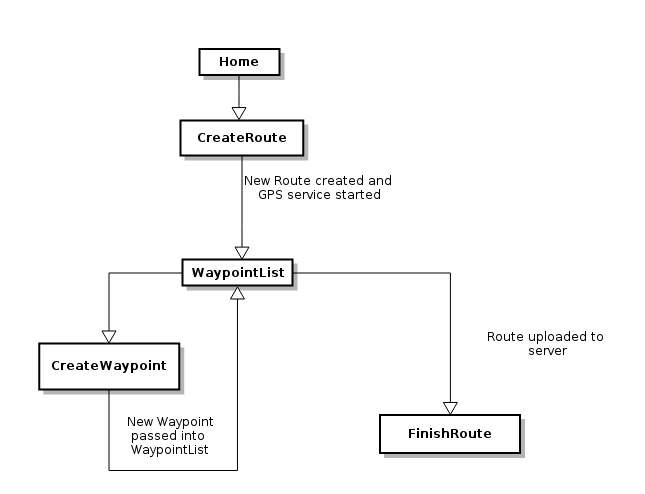
\includegraphics[width=\columnwidth]{img/data_flow}
			\end{center}
		\end{subsection}
	\end{section}
	
	\newpage
	\begin{section}{Data Classes}
		This section details the significant or complex methods and data structures in each class - large parts of the code base are very well-commented and self-explanatory, so it is only the more complex areas that are mentioned in this document.
		\begin{subsection}{StumblrData}
			\begin{subsubsection}{Significant methods}
				\begin{itemize}				
					\item{{\bf public string sanitiseStringInput} \\
					This method takes a String object and replaces all forbidden characters (more specifically, characters that do not belong to the set "a-z", "A-Z", "0-9", ",.!?:;" and "-". This ensures that String data is safe to transmit to the web server.}
				\end{itemize}
			\end{subsubsection}
		\end{subsection}
	
		\begin{subsection}{Route}
			The Route class is the main container for the metadata of the walk - including the description, timestamps, the list of coordinates for the breadcrumb trail, and the list of Waypoints (a datatype that will be covered further later in this document). \\
			
			\begin{subsubsection}{Significant data structures}
				\begin{itemize}				
					\item{{\bf private Stack<Location> coordinates;} \\
					This holds the "breadcrumb trail" - a Stack of Location objects (from the Android API). This is where the Location objects are stored when they are obtained from the GPSService class. Location objects are passed from the GPSService class by using Broadcastsm and then filtering by intent. (This is covered in detail later).}
					\item{{\bf private LinkedList<Waypoint> route;} \\
					This holds the list of Waypoint objects - including an instance of a Bitmap image (from the Android API), and Strings relating to the title and description of the Waypoint.}
				\end{itemize}
			\end{subsubsection}
			
			\begin{subsubsection}{Significant methods}
				\begin{itemize}
					\item{{\bf public float getDistance} \\
					This method calculates the cumulative distance between all of the "breadcrumbs" in the 'coordinates' Stack. The method loops through the list and calls the Android API method {\bf Location.distanceBetween()} on each successive pair of coordinates,. Returns a {\bf float} containing the total distance between each pair of coordinates.}
					
					\item{{\bf public void writeToParcel} \\
					Writes the current contents of the Route object to a {\bf Parcel} object (Android API), to allow the Route to be passed between Activities. Required for implementing the {\bf Parcelable} interface.}
					
					\item{{\bf public void readFromParcel} \\
					Reads a Parcel into the current Route object. Required for implementing the {\bf Parcelable} interface.}
				\end {itemize}
			\end{subsubsection}
		\end{subsection}
		
		\newpage
		\begin{subsection}{Waypoint}
			\begin{subsubsection}{Significant methods}
				\begin{itemize}
					\item{{\bf public void writeToParcel} \\
					Writes the current contents of the Waypoint object to a {\bf Parcel} object (Android API), to allow the Route to be passed between Activities. Required for implementing the {\bf Parcelable} interface.}
					
					\item{{\bf public void readFromParcel} \\
					Reads a Parcel into the current Waypoint object. Required for implementing the {\bf Parcelable} interface.}
				\end {itemize}
			\end{subsubsection}
		\end{subsection}
	\end{section}
	
	\begin{section}{Activity Classes}
		\begin{subsection}{AbstractActivity}
			This class contains all of the common code elements that are used in the other Activities. This includes the code that display the "cancel confirmation" alert dialogue. This class is largely self-explanatory.
		\end{subsection}
		
		\begin{subsection}{CreateRoute}
			\begin{subsubsection}{Significant methods}
				\begin{itemize}
					\item{{\bf public void startWaypointListIntent} \\
					This starts the WaypointList Activity after checking that the input fields of the Activity are the correct length.}
				\end{itemize}
			\end{subsubsection}
		\end{subsection}
		
		\begin{subsection}{CreateWaypoint}
			This Activity is called from the WaypointList activity - and this is where the user can create Waypoints to correspond with Points of Interest (POIs) during the walk.
			\begin{subsubsection}{Significant methods}
				\begin{itemize}
					\item{{\bf public void stumblrOnCreate} \\
					This method is essentially the Activity's constructur - it checks the Bundle data passed into the Activity - checking for a Location object or a Waypoint object. The object is then loaded into the appropriate instance variables (depending on the type). The last thing this method does is use the Android API to check if certain capabilities are enabled; namely, a camera and gallery.}
					
					\item{{\bf public void finishWaypoint} \\
					This just validates the data entered on-screen, warning the user with a {\bf Toast} if any data entered is invalid. A timestamp is then applied to the current Waypoint, and the Waypoint object is put into a Bundle as a return value for the Activity - this Bundle is returned to WaypointList (as it is instantiated with {\bf startActivityForResult()}).}
					
					\item{{\bf public void getImage} \\
					Gets an image from user's camera or gallery, after checking which is available. An Activity is dispatched (based upon what is available) using {\bf startActivityForIntent}.}
					
					\item{{\bf protected void onActivityResult} \\
					This method handles return values from the camera or gallery Activities dispatched in the previous method. Depending on the activity that returned the image, it will be resized and cast to a {\bf Bitmap} for easy conversion to Base64, and submission (via JSON) to the web server.}
				\end{itemize}
			\end{subsubsection}
		\end{subsection}
		
		\newpage
		\begin{subsection}{FinishRoute}
		This Activity is responsible for converting the (completed) Route object to JSON and uploading it to the web server, ready for displaying on the web interface. As the data structures dealt with in this class are generally 
			\begin{subsubsection}{Significant methods}
				\begin{itemize}
					\item{{\bf public void stumblrOnCreate} \\
					This method is fairly simple - it unbundles the Route object from the extras passed in from the calling Intent, and puts it into memory. The remaining Route metadata is then calculated and displayed onscreen.}
					\item{{\bf public void postData} \\
					This method simply uses the Android API to check if the device has an internet connection - if so, the NetworkTast is executed, and the data is sent.}
					
					\item{{\bf public JSONObject getData} \\
					This converts the Route object into JSON ready for transmission to the web server. This method uses the {\bf JSONObject (org.json.JSONObject)} class from the standard Java JSON libraries.}
					
					\item{{\bf public String encodeToBase64} \\
					This is fairly simple - a {\bf ByteArrayOutputStream} decodes a {\bf Bitmap} object into raw data - which is then encoded using Base64}
				\end{itemize}
			\end{subsubsection}
		\end{subsection}
		
		\begin{subsection}{GPSService}
			GPSService uses a Foreground Notification (to avoid getting killed by Android) and implements {\bf LocationListener} so that it is able to subscribe to Location update (provided by GPS). The {\bf Location} objects are then sent back to the main Activity by using a Broadcast.
			\begin{subsubsection}{Significant methods}
				\begin{itemize}
					\item{{\bf public int onStartCommand} \\
					This is a rather straightforward method, but it looks a little complicated. It subscribes the current class to receive {\bf Location} updates and places a persistent {\bf Notification} in the user's Notification Centre. {\bf Be aware: There is officially deprecated code inside this method so that the persistent Notification can be shown on older versions of Android.}}
					\item{{\bf public void onDestroy} \\
					This method tells the class to stop receiving Location updates when killed - this ensures that the device's battery is not wasted.}
					\item{{\bf public void onLocationChanged} \\
					This method is very simple, but its function may not be immediately obvious. It is called when a {\bf Location} update is received by the {\bf GPSService} class, and it bundles the received {\bf Location} object and sends it as a {\bf Broadcast} to the system, where the message is picked up by {\bf WaypointList} and added to the current Waypoint.}
				\end{itemize}			
			\end{subsubsection}
		\end{subsection}
		
		\begin{subsection}{Home}
			The Home class contains no complex methods as it is approximately 35 lines in length and only contains code for one button!
		\end{subsection}
		
		\newpage
		\begin{subsection}{WaypointList}
			This is the main Activity of the application in that most of the user's time is spent using it. From this Activity, the user can view, add to, and edit the current list of Waypoints. The user can also decide to complete the walk, dispatching the FinishRoute Activity.
			\begin{subsubsection}{Significant data structures}
				\begin{itemize}
					\item{{\bf private ListView listView} \\
					This ListView object is used to display and manipulate the Route's Waypoints on-screen. The user can view a list of the current Waypoints, or edit the}
				\end{itemize}
			\end{subsubsection}
			
			
			\begin{subsubsection}{Significant methods}
				\begin{itemize}
					\item{{\bf protected void onActivityResult} \\
					This method is called when a dispatched Activity (in this case, CreateWaypoint) exits and returns with a valid Waypoint object - the new Waypoint is added to the list and the ListView is refreshed.}
					
					\item{{\bf private void startGPSService} \\
					There is a private class declaration within this method that contains methods to add coordinates received from the GPSService to the current trail of {\bf Locations}. If GPS is disabled, the method prompts the user to enable it.}
					
					\item{{\bf public void onDestroy} \\
					Called before the Activity is destroyed (part of the Android application lifecycle). This sends a signal to the running GPS service to halt and exit (thus removing the {\bf Notification} at the top of the user's screen).}
				\end{itemize}
			\end{subsubsection}
		\end{subsection}
	\end{section}
	
	\begin{section}{Limitations of the Application}
		There are a number of limitations to the application in question, the principal of which are the Android API versions that it supports. Currently, the application supports (and has been fully tested on) API/SDK versions {\bf 8} to {\bf 22} - which correlates to Android versions {\bf 2.2} through {\bf 4.4}. \\
		
		There are also a number of important considerations when it comes to battery and memory usage. Each Waypoint (including thumbnail image) is stored entirely in working memory (RAM) - theoretically, this limits the number of Waypoints that a low-RAM device can hold; although in practice, the amount of data in memory (even on large walks) is relatively small, and memory usage is a very minor consideration. Certainly, we experienced no issues on an older Android {\bf 2.3} device with severe memory limitations, with walks of 20 Waypoints and above. \\
		
		The application is also rather battery intensive on longer walks; the GPS service, while being useful for regularly fetching location data - uses an enormous amount of battery power, particularly if the GPS signal is bad (due to overcast weather, large buildings in the surrounding area, etc). This is sufficient to flatten some more power-hungry devices with 5-6 hours' usage (tested overnight on a tablet device).
	\end{section}
	
	\begin{section}{Interaction with Remote Server}
		The interaction with the server is kept as simple as possible. The Java objects created within the application are converted to JSON (a human-readable format useful when transmitting complex objects), and transferred to the server via HTTP POST. The HTTP interaction is completed with the Apache Commons HTTP libraries, and the code used to interact with the server is currently in the FinishRoute class.
	\end{section}
	
	\newpage
	\begin{section}{Building and Testing}
		This section details the tools and methods that were used to create and compile the application and documentation.
		
		\begin{subsection}{Building}
			The build tools used in the creation of the Java code base were Android Studio, coupled with the Gradle build system. The supplementary files inside the Git repository are mostly to ensure proper functioning of Gradle and the Android Studio IDE.
		\end{subsection}
		
		\begin{subsection}{Testing}
			The testing code for this assignment was written using JUnit - a testing suite that complements the Java language.
		\end{subsection}
		
		\begin{subsection}{Documentation}
			All documentation for this project (where possible) has been written and rendered using \LaTeX. \LaTeX can be a challenge to write for new users, so a procedure was defined for team members who struggle getting it to work; writing documents in MarkDown and then converting them. MarkDown is a minimal, intuitive markup language (also used on GitHub for formatting text files) that aims to be easy to write. This was excellent for our needs, as MarkDown syntax can be easily converted to \LaTeX syntax using a system like PanDoc. \\ \\
			Markdown: \url{https://daringfireball.net/projects/markdown/} \\
			PanDoc: \url{http://johnmacfarlane.net/pandoc/}
		\end{subsection}
		
		\begin{subsection}{References to external sources}
			References to external sources are usually contained inside inline comments in the Java code; {\em for example}: \\ \\
			{\tt // See: somewebsite.com/url/resource.html}
		\end{subsection}
	\end{section}
	
	% Include references here (edit the References.bib file)
	\nocite{LaTeXTemplate} % DO NOT EDIT

	% Format bibliography/refs
	\newpage
	\begin{section}{REFERENCES}
		\bibliographystyle{acm}
		\bibliography{References}
	\end{section}
	
	\vspace{1cm}
	\begin{section}{VERSION HISTORY}
		\versionhistory
	\end{section}
\end{document}

%									Useful bits and pieces
%\begin{section}{section_name}								% Start section
%\end{section}												% End section
%\begin{center} \end{center}								% Center stuff
%\includegraphics[width=0.75\columnwidth]{example_figure}	% Insert image
%\pseudocode{filename}{caption}								% Insert highlighted code snippet
%\clearpage													% Clear page after section
%\url{http://www.google.com/} 								% Include URL
%\nocite{citationName}										% Cite to bibliography (but not to text)
%\cite{citationName}										% Include reference